\chapter{Methodology}
\label{ch:methodology}

This chapter describes the design and implementation of a software pipeline for the semantic sorting of transparent plastic waste. The system addresses two obstacles that jointly prevent the direct application of existing robotic manipulation methods to this domain: active infrared depth sensors return corrupted or missing measurements over transparent surfaces, and no large-scale dataset of language-annotated robot demonstrations exists for transparent waste items.

The pipeline is organised as a cascade of three components, developed as separate work packages. Work Package 1 (WP1) is a procedural data generation framework, referred to as ReSort-IT, which synthesises image--language--action training triplets from existing transparent-object assets without requiring physical robot demonstrations. Work Package 2 (WP2) is a multi-task convolutional network that predicts surface normals and segmentation masks from RGB input, feeding a depth reconstruction solver that repairs the corrupted sensor stream. Work Package 3 (WP3) fine-tunes a pre-trained 7-billion-parameter Vision-Language-Action model~\citep{kim2024} on the synthetic data using parameter-efficient adaptation. The chapter closes with the evaluation methodology used to assess each component and the integrated system.

A cascaded design was chosen over end-to-end training for three reasons. First, it decouples metric depth recovery from semantic reasoning, so each component can be evaluated, debugged, and replaced independently. Second, it keeps the large language-model backbone isolated from geometric computation, for which it is poorly suited. Third, it permits the perception front-end and the policy to be trained on different data sources, which is necessary because ground-truth geometry (normals, depth) and action labels come from different generation processes.

\begin{figure}[htbp]
    \centering
    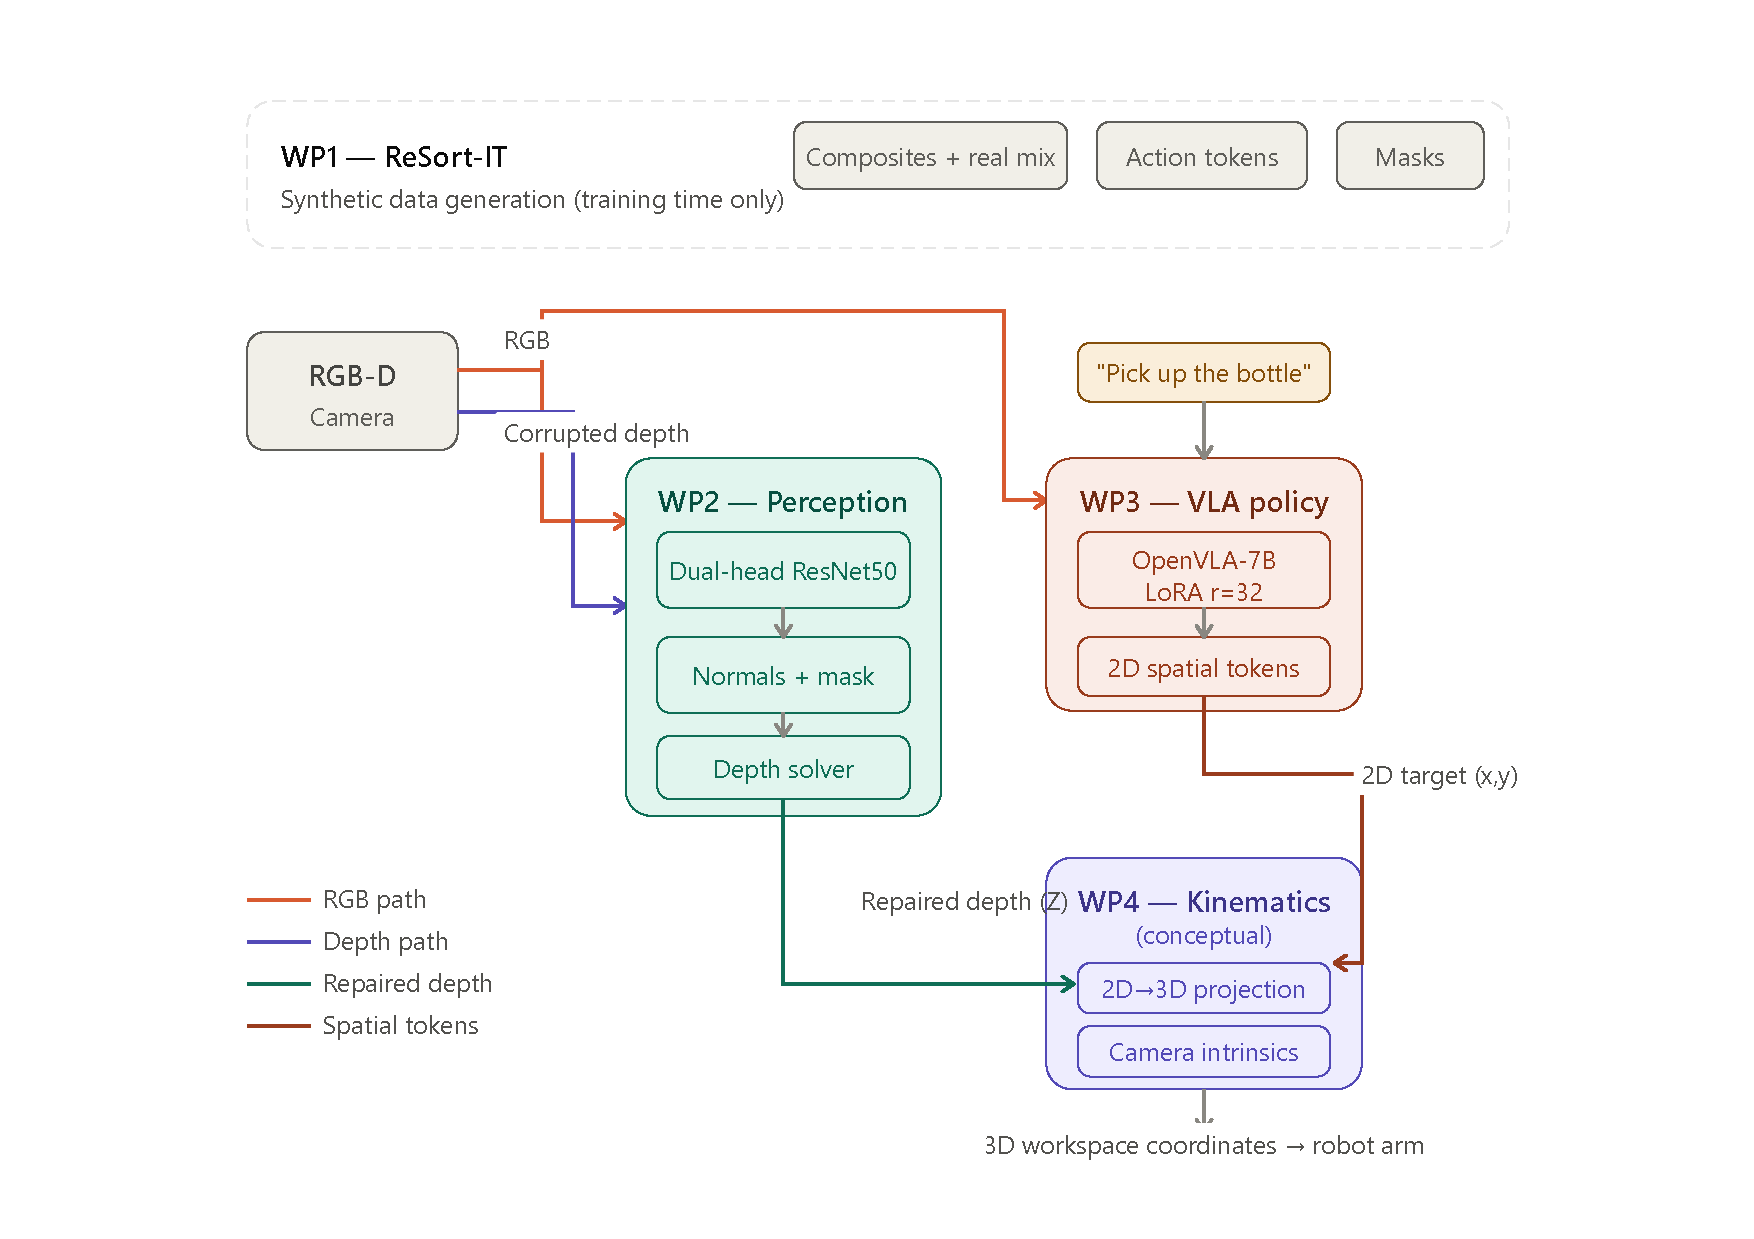
\includegraphics[width=\textwidth]{images/vla_architecture_diagram.pdf}
    \caption{End-to-end system architecture. The WP2 perception module provides repaired metric depth, which combines with the WP3 VLA policy's 2D spatial tokens to yield 3D workspace coordinates via WP4 kinematics.}
    \label{fig:architecture}
\end{figure}

\section{Work Package 1: Synthetic Data Generation (ReSort-IT)}
\label{sec:wp1}

\subsection{Source Assets}
\label{subsec:source_assets}

Foreground objects were sourced from the ClearGrasp synthetic dataset~\citep{sajjan2020}, which provides photorealistic renders of transparent plastic objects with per-pixel segmentation masks, surface normals, and depth. The \texttt{square-plastic-bottle} category, comprising 11{,}702 RGB--mask pairs, was used to train the manipulation policy. Background plates were drawn from a separately collected pool of 153 texture images spanning industrial and domestic surfaces (conveyor rubber, wood, concrete, fabrics, and patterned materials).

A deliberate scoping decision was made to restrict policy training to a single object category. This isolates the central research question---whether a VLA can learn spatial grounding of transparent objects from composited synthetic data---from the separate question of multi-class generalisation. The remaining ClearGrasp categories were reserved as held-out data for evaluating the generalisation of the perception module (Section~\ref{sec:eval_methodology}).

\subsection{Grasp Target Derivation}
\label{subsec:target_derivation}

Each ClearGrasp render may contain several disconnected transparent objects. Deriving a grasp target from the centroid of the full mask fails in this situation: averaging over multiple objects places the target in the empty space between them, a failure mode observed during early development and referred to here as the \emph{empty-centre} problem. On a physical sorting line this would direct the end-effector into the bare conveyor surface.

To resolve this, individual objects are first isolated by connected-component analysis. The binary mask $\mathbf{M}$ is decomposed into external contours,
\begin{equation}
    \mathcal{C} = \{c_1, \dots, c_n\} = \mathrm{findContours}(\mathbf{M}),
\end{equation}
and one contour $c_i$ is selected uniformly at random as the grasp target for that composite; the remaining objects are retained in the frame as clutter. The target coordinate is then the centre of mass of the selected contour, computed from its image moments,
\begin{equation}
    M_{pq} = \sum_{(x,y) \in c_i} x^{p} y^{q}, \qquad
    c_x = \frac{M_{10}}{M_{00}}, \quad c_y = \frac{M_{01}}{M_{00}},
\end{equation}
which places the ground-truth target on solid object material rather than in
the gap between objects for convex shapes. The centroid guarantee does not,
however, hold for concave objects: for crescent-shaped or crushed items, the
centre of mass can fall outside the object entirely. An audit of the first
generated dataset (Section~\ref{subsec:res_labelaudit}) found that 10\% of
targets suffered exactly this defect. The final generator therefore validates
every centroid with a point-in-polygon test,
\begin{equation}
    \mathrm{pointPolygonTest}(c_i, (c_x, c_y)) \geq 0,
\end{equation}
and, where the test fails, substitutes the contour's most-interior point---the
argmax of the L2 distance transform of the filled contour---which lies on
object material by construction. A runtime assertion additionally verifies
every emitted label against its saved object mask, so label validity in the
final dataset is 100\% by construction rather than by expectation.

\subsection{Compositing and Domain Randomisation}
\label{subsec:compositing}

Each source image is composited onto randomly selected backgrounds three times, with independently sampled transformations, yielding 35{,}103 composites in total for the initial baseline dataset (Run 1). The following randomisations are applied to every composite:

\begin{itemize}
    \item \textbf{Scale.} The foreground is resized so that its width is a fraction $s \sim \mathcal{U}(0.25, 0.75)$ of the 640-pixel background width, covering both distant and close object appearances.
    \item \textbf{Geometric transforms.} A horizontal flip is applied with probability $0.5$, followed by a rotation of $\theta \sim \mathcal{U}(-15^{\circ}, 15^{\circ})$. The mask is re-thresholded after rotation to remove interpolation artefacts.
    \item \textbf{Photometric jitter.} Foreground contrast is scaled by $\alpha \sim \mathcal{U}(0.6, 1.4)$ and brightness shifted by $\beta \sim \mathcal{U}(-40, 40)$; in HSV space, hue is shifted by up to $\pm 10^{\circ}$ and saturation scaled by $\mathcal{U}(0.7, 1.3)$.
    \item \textbf{Edge softening.} The binary mask is blurred with a $7 \times 7$ Gaussian kernel before alpha blending. This removes the sharp compositing seam at the object boundary, which would otherwise provide the network with a localisation shortcut unrelated to object appearance.
    \item \textbf{Sensor noise.} Zero-mean Gaussian noise with $\sigma \sim \mathcal{U}(1, 5)$ intensity levels is added to the final composite.
    \item \textbf{Position.} The composite location is sampled uniformly subject to the object remaining fully in frame, and independently of the background identity, so that no correlation exists between background appearance and target position.
\end{itemize}

Alpha blending with the softened mask $\tilde{\mathbf{M}}$ produces the final composite:
\begin{equation}
    \mathbf{I}_{\mathrm{comp}} = \mathbf{I}_{\mathrm{fg}} \odot \frac{\tilde{\mathbf{M}}}{255} + \mathbf{I}_{\mathrm{bg}} \odot \left(1 - \frac{\tilde{\mathbf{M}}}{255}\right).
\end{equation}

\subsection{Real-Frame Mixing and Native Resolution}
\label{subsec:realframe_mixing}
 
Two properties of the first-generation dataset were identified as root causes
of the spatial-precision ceiling measured in Chapter~4, and the final dataset
corrects both.
 
First, alpha compositing removes precisely the cues by which transparent
objects are localised in real images: refraction of the background through the
object, cast and contact shadows, and physically consistent specular
highlights. A pasted transparent object looks identical regardless of what
lies behind it, so no training signal links object position to
transparency-specific appearance. The final dataset therefore mixes two
sources in roughly equal proportion: each source image contributes two
composites \emph{and} two lightly augmented native ClearGrasp frames
(horizontal flip, photometric jitter, and sensor noise only---no rotation,
preserving the authentic render geometry), labelled from their own
segmentation masks with the validity-guaranteed target derivation of
Section~\ref{subsec:target_derivation}. The native frames carry true
refraction and shadowing; the composites carry background diversity.
 
Second, the first-generation samples were rendered at $640 \times 480$ and
subsequently resized to the policy's $224 \times 224$ encoder input,
compounding two lossy resamplings. The final dataset is generated directly at
$224 \times 224$, so objects are downsampled once, under controlled
interpolation. At this resolution one action bin corresponds to $0.875$
pixels, so tokenisation granularity is no longer a limiting factor on
achievable precision.
 
\begin{table}[htbp]
    \centering
    \caption{Final (Run~2) dataset composition by split and sample type.}
    \label{tab:run2_dataset}
    \begin{tabular}{lccc}
        \toprule
        \textbf{Split} & \textbf{Composites} & \textbf{Native frames} & \textbf{Total} \\
        \midrule
        Train      & 14{,}470 & 16{,}380 & 30{,}850 \\
        Validation &  3{,}110 &  3{,}510 &  6{,}620 \\
        Test       &  3{,}095 &  3{,}512 &  6{,}607 \\
        \midrule
        \textbf{Total} & \textbf{20{,}675} & \textbf{23{,}402} & \textbf{44{,}077} \\
        \bottomrule
    \end{tabular}
\end{table}
 

\subsection{Real-Frame Mixing and Native Resolution}
\label{subsec:realframe_mixing}
 
Two properties of the first-generation dataset were identified as root causes
of the spatial-precision ceiling measured in Chapter~4, and the final dataset
corrects both.
 
First, alpha compositing removes precisely the cues by which transparent
objects are localised in real images: refraction of the background through the
object, cast and contact shadows, and physically consistent specular
highlights. A pasted transparent object looks identical regardless of what
lies behind it, so no training signal links object position to
transparency-specific appearance. The final dataset therefore mixes the two
sources in equal proportion: each source image contributes two composites
\emph{and} two lightly augmented native ClearGrasp frames (horizontal flip,
photometric jitter, and sensor noise only---no rotation, preserving the
authentic render geometry), labelled from their own segmentation masks with
the validity-guaranteed target derivation of
Section~\ref{subsec:target_derivation}. The native frames carry true
refraction and shadowing; the composites carry background diversity. The
resulting split comprises approximately equal numbers of each
(Table~\ref{tab:run2_dataset}).
 
Second, the first-generation samples were rendered at $640 \times 480$ and
subsequently resized to the policy's $224 \times 224$ encoder input,
compounding two lossy resamplings. The final dataset is generated directly at
$224 \times 224$, so objects are downsampled once, under controlled
interpolation. At this resolution one action bin corresponds to $0.875$
pixels, so tokenisation granularity is no longer a limiting factor on
achievable precision.
\begin{table}[htbp]
    \centering
    \caption{Final (Run-2) dataset composition. Counts per split
    \textbf{[TBD --- fill from the generator's summary output]}.}
    \label{tab:run2_dataset}
    \begin{tabular}{lccc}
        \toprule
        \textbf{Split} & \textbf{Composites} & \textbf{Native frames} & \textbf{Total} \\
        \midrule
        Train & [TBD] & [TBD] & [TBD] \\
        Validation & [TBD] & [TBD] & [TBD] \\
        Test & [TBD] & [TBD] & [TBD] \\
        \bottomrule
    \end{tabular}
\end{table}

\subsection{Data Partitioning}
\label{subsec:partitioning}

Leakage between splits was controlled at two levels. Source images were partitioned 70/15/15 into train, validation, and test sets before compositing, so no rendered object instance appears in more than one split. Independently, the 153 background plates were partitioned with the same ratios (107/22/24), and each split draws backgrounds exclusively from its own pool. Without this second control, a model could achieve low validation error by recognising a background seen during training. 
The resulting initial dataset (Run 1) comprises 24,570 training, 5,265 validation, and 5,268 test composites. The composition of the final dataset (Run 2), which incorporates native frames, is detailed in Section 3.1.4 and Table 3.1.
\subsection{Action Representation and Tokenisation}
\label{subsec:action_tokens}

Each composite is paired with a natural-language instruction (``Pick up the transparent plastic bottle.'') and a 7-dimensional action vector following the OpenVLA convention: planar target coordinates $(x, y)$, height $z$, orientation (roll, pitch, yaw), and gripper state. The target coordinates are normalised by the image dimensions; the remaining dimensions are fixed at neutral values ($z = \mathrm{roll} = \mathrm{pitch} = \mathrm{yaw} = 0.5$, gripper~$= 1.0$), reflecting the top-down grasp geometry of a conveyor workspace in which only the planar target varies between samples.

Because the language-model backbone operates on discrete tokens, each continuous dimension $a \in [0, 1]$ is quantised into 256 uniform bins,
\begin{equation}
    a_{\mathrm{quant}} = \mathrm{clip}\!\left(\mathrm{round}(255\,a),\, 0,\, 255\right),
\end{equation}
and mapped to a reserved vocabulary token $\langle \mathrm{action}\_k \rangle$, $k \in \{0, \dots, 255\}$. One bin therefore corresponds to $2.5$ pixels horizontally and $1.9$ pixels vertically at the $640 \times 480$ working resolution. The complete training sample is the prompt
\begin{quote}
\texttt{In: What action should the robot take to \{instruction\}\textbackslash n Out: $\langle$action\_$x\rangle$ $\langle$action\_$y\rangle$ \dots $\langle$action\_$g\rangle$}
\end{quote}
paired with the composite image.

\section{Work Package 2: Perception Front-End}
\label{sec:wp2}

\subsection{Network Architecture}
\label{subsec:architecture}

The perception module is a dual-head fully convolutional network built on DeepLabV3~\citep{chen2017rethinking} with an ImageNet-pretrained ResNet-50 backbone. The backbone and the Atrous Spatial Pyramid Pooling stage are shared; the final classifier is replaced by two parallel $1 \times 1$ convolutional heads operating on the shared 256-channel feature map:

\begin{enumerate}
    \item a \textbf{surface-normal head} producing a 3-channel map, L2-normalised along the channel dimension so that every pixel emits a unit vector $\hat{\mathbf{n}} = [n_x, n_y, n_z]^{\top}$; and
    \item a \textbf{segmentation head} producing 1-channel logits for the transparent-versus-background decision.
\end{enumerate}

Both outputs are bilinearly upsampled to the input resolution within the forward pass. Training and evaluation use $256 \times 256$ inputs; at inference the fully convolutional design permits arbitrary resolutions.

\subsection{Loss and Optimisation}
\label{subsec:loss}

The normal head is trained with a cosine similarity loss over all pixels,
\begin{equation}
    \mathcal{L}_{\mathrm{normals}} = 1 - \frac{1}{N} \sum_{i=1}^{N}
    \frac{\hat{\mathbf{n}}_i \cdot \mathbf{n}_i}{\lVert\hat{\mathbf{n}}_i\rVert_2\,\lVert\mathbf{n}_i\rVert_2},
\end{equation}
and the segmentation head with binary cross-entropy on logits, $\mathcal{L}_{\mathrm{mask}}$. The joint objective is the unweighted sum $\mathcal{L} = \mathcal{L}_{\mathrm{normals}} + \mathcal{L}_{\mathrm{mask}}$; no weighting search was performed, as both losses converged at comparable scales. The network was trained for 10 epochs with AdamW (learning rate $10^{-4}$, batch size 4) on the \texttt{square-plastic-bottle} category, using the ClearGrasp-provided normals and masks as supervision.

\subsection{Depth Reconstruction Solver}
\label{subsec:solver}

The predicted normals and mask feed a global optimisation that reconstructs metric depth over the transparent regions, following the strategy introduced by ClearGrasp~\citep{sajjan2020}: depth values on the opaque background, where the sensor is reliable, act as boundary anchors, and the predicted normals constrain the surface gradients inside the missing region.

Under the pinhole camera model, the depth gradient in pixel coordinates $(u, v)$ relates to the surface normal as
\begin{equation}
    \frac{\partial Z}{\partial u} = -\frac{n_x\, Z}{n_z\, f_x}, \qquad
    \frac{\partial Z}{\partial v} = -\frac{n_y\, Z}{n_z\, f_y},
    \label{eq:perspective_gradients}
\end{equation}
where $f_x, f_y$ are the focal lengths in pixels. The dependence on the unknown depth $Z$ is resolved by approximating it with the mean depth $\bar{Z}$ of the valid pixels in a two-pixel dilated band around the hole, which is accurate when the object's depth extent is small relative to its distance from the camera---the operating regime of a fixed overhead sensor. ClearGrasp renders use Intel RealSense D415 intrinsics ($f_x = f_y = 918$ at $1920 \times 1080$); focal lengths are scaled proportionally when images are downsampled. Omitting the $1/f$ scaling in Equation~\ref{eq:perspective_gradients} inflates the gradient targets by more than two orders of magnitude and causes the solver to diverge; this correction proved essential during development.

Let $\Omega$ denote the hole region (the predicted mask union any zero-depth pixels). The reconstruction $\mathbf{D}$ is the least-squares solution of a sparse linear system containing three families of equations: finite-difference gradient constraints in $u$ and $v$, imposed only on pixel pairs of which at least one member lies in $\Omega$; and anchor constraints
\begin{equation}
    \lambda\, D(u, v) = \lambda\, D_{\mathrm{raw}}(u, v), \qquad (u, v) \notin \Omega,
\end{equation}
with anchor weight $\lambda = 100$. Restricting gradient constraints to the hole region and weighting the anchors strongly prevents small inconsistencies between predicted normals and true background geometry from perturbing the reliable measurements---an effect that, in unrestricted formulations, degraded the reconstruction below the accuracy of the raw corrupted input. The system is solved with the iterative LSQR method on a compressed sparse-row matrix, and the output is clipped to the physically valid range $[0, 2.5]$\,m. The sensitivity of the reconstruction to the choice of $\lambda$ is quantified empirically in Chapter~4.

One implementation detail warrants documentation: OpenCV loads the ClearGrasp EXR normal maps in BGR channel order, so the stored channels correspond to $(n_z, n_y, n_x)$ rather than $(n_x, n_y, n_z)$. The channel reordering must be applied to both ground-truth and predicted normals before Equation~\ref{eq:perspective_gradients}; omitting it silently exchanges the $x$ and $z$ components and produces divergent reconstructions.

\section{Work Package 3: VLA Fine-Tuning}
\label{sec:wp3}

\subsection{Base Model}
\label{subsec:base_model}

The manipulation policy is OpenVLA-7B~\citep{kim2024}, an open-source Vision-Language-Action model that maps an RGB observation and a language instruction to discrete action tokens. Its vision stack fuses SigLIP and DINOv2 encoders, whose complementary features (global semantics and fine-grained spatial structure respectively) are projected into the embedding space of a Llama-2 7B language backbone; actions are generated autoregressively as text tokens. OpenVLA was selected over closed alternatives such as RT-2~\citep{zitkovich2023} because its weights, tokeniser, and action vocabulary are publicly available, which the fine-tuning and evaluation protocols in this work require.

\subsection{Parameter-Efficient Adaptation}
\label{subsec:lora}

Full fine-tuning of a 7B-parameter model is infeasible on the available hardware (a single NVIDIA A100) and risks catastrophic forgetting of the pre-trained visuomotor priors. Low-Rank Adaptation~\citep{hu2021lora} is used instead: the pre-trained weights $\mathbf{W}_0$ are frozen, and trainable low-rank updates are added to the query and value projections of every attention layer,
\begin{equation}
    \mathbf{W} = \mathbf{W}_0 + \frac{\alpha}{r}\,\mathbf{B}\mathbf{A},
    \qquad \mathbf{A} \in \mathbb{R}^{r \times k},\;
    \mathbf{B} \in \mathbb{R}^{d \times r},
\end{equation}
with rank $r = 32$, scaling $\alpha = 32$, and dropout $0.05$. This yields $16{,}777{,}216$ trainable parameters, $0.22\%$ of the $7.56 \times 10^{9}$ total. To fit within GPU memory alongside optimiser state, the frozen base weights are stored in 4-bit NormalFloat (NF4) quantisation~\citep{dettmers2023qlora} while forward and backward computation is performed in \texttt{bfloat16}.

\subsection{Training Protocol}
\label{subsec:training_protocol}

Loss masking restricts supervision to the action tokens. For each sample, the label sequence is a copy of the input token sequence in which every position preceding the action tokens (the instruction prompt) and every padding position is set to the ignore index $-100$, so the cross-entropy loss is computed over exactly the seven action tokens. Without this masking, the loss is dominated by trivially predictable prompt text, which dilutes the gradient signal on the coordinates that constitute the task.

Training used a batch size of 2 with AdamW at a learning rate of $10^{-5}$ for a maximum of 5 epochs. Validation loss was computed every 500 optimisation steps on a fixed subset of the validation split, with early stopping after 15 consecutive evaluations without improvement and checkpointing of the best-performing adapter. Continuous validation monitoring was adopted after a preliminary experiment demonstrated that, in the absence of such monitoring, memorisation of the training composites can proceed undetected: training loss alone reached machine zero while spatial accuracy on held-out data remained at chance level. This failure mode and its diagnosis are analysed in Chapter~4. In the final run, training halted at step 21{,}500 (during the second epoch) with a best validation loss of $0.154$.

\section{Evaluation Methodology}
\label{sec:eval_methodology}

The evaluation is organised around four questions: (i)~how accurately does the perception module recover geometry, both on the training category and on unseen object categories; (ii)~does normal-guided depth reconstruction outperform geometry-unaware baselines, and by how much does prediction error in the normals degrade the reconstruction; (iii)~how accurately does the fine-tuned policy localise grasp targets, and does that accuracy translate into physically plausible grasp points; and (iv)~what is the computational cost of the pipeline per frame.

\subsection{Perception Metrics}
\label{subsec:perception_metrics}

Surface-normal quality is reported as the mean, median, and root-mean-square angular error in degrees over object pixels, together with the standard threshold accuracies (the fraction of pixels with error below $11.25^{\circ}$, $22.5^{\circ}$, and $30^{\circ}$). Segmentation is reported as mean intersection-over-union. All metrics are computed in-distribution on the training category and out-of-distribution on two held-out ClearGrasp categories (\texttt{cup-with-waves} and \texttt{stemless-plastic-champagne-glass}) that the network never observed, providing a direct measure of shape generalisation.

\subsection{Depth Reconstruction Ablation}
\label{subsec:ablation_design}

Sensor failure is simulated by setting the ground-truth depth to zero over the object mask, so that the true depth of the corrupted region is known exactly. Four recovery conditions are compared on 100 images at half resolution: (A)~the raw corrupted depth; (B)~Navier--Stokes inpainting (\texttt{cv2.inpaint}), a texture interpolation baseline with no knowledge of 3D geometry; (C)~the Poisson solver of Section~\ref{subsec:solver} driven by ground-truth normals, which upper-bounds the achievable reconstruction; and (D)~the same solver driven by the normals predicted by WP2, which is the deployed configuration. Errors (RMSE, MAE, and mean relative error, in metres) are computed exclusively over the corrupted region.

Because the four conditions are evaluated on the same images, differences are tested with the paired Wilcoxon signed-rank test, which does not assume normally distributed errors, and each condition's mean RMSE is reported with a bootstrap 95\% confidence interval ($10^{4}$ resamples). The anchor weight is additionally swept over $\lambda \in \{10, 50, 100, 500, 1000\}$ on a 30-image subset to establish the sensitivity of the reconstruction to this hyperparameter.

\subsection{Policy Metrics}
\label{subsec:policy_metrics}

Policy accuracy is measured on the held-out validation split by autoregressive generation: the model receives the image and the instruction prompt and generates action tokens, which are decoded back to coordinate bins. The primary metric is the mean L1 error in bins between predicted and ground-truth coordinates, reported per axis and in aggregate, alongside exact-match token accuracy. Aggregate token accuracy is treated with caution: five of the seven action dimensions are constants in this task, so a policy can achieve high aggregate accuracy while failing entirely on the two coordinates that matter. Per-axis coordinate error is therefore the headline measure. Accuracy is tracked across all training checkpoints to characterise the learning trajectory.

To connect bin-space error to task feasibility, a grasp-success proxy is computed: a prediction is counted as successful if it falls within a fixed radius of the ground-truth grasp point, and the success rate is reported with a Wilson 95\% confidence interval. This proximity criterion is conservative---a prediction landing on the object but far from its centroid is counted as a failure---and the implications of this choice are discussed with the results.

\subsection{Runtime Profiling}
\label{subsec:runtime}

End-to-end latency is profiled on the A100 by timing each stage (perception forward pass, sparse depth reconstruction, and VLA generation) over 20 runs after warm-up, with CUDA synchronisation around GPU stages. The results identify which component bounds the throughput of the pipeline and quantify the distance to conveyor-rate operation.

\section{Implementation and Hardware}
\label{sec:implementation}

All components were implemented in Python using PyTorch, HuggingFace Transformers and PEFT, OpenCV, and SciPy. Dataset generation runs on CPU; perception training, VLA fine-tuning, and all GPU evaluation ran on a single NVIDIA A100 on the university compute cluster, accessed through a jump host with sessions persisted in \texttt{tmux}. The complete VLA fine-tuning run required approximately 21{,}500 optimisation steps; the depth reconstruction solver processes a $960 \times 540$ frame in approximately 2.5\,s on CPU.

\section{Summary}
\label{sec:method_summary}

This chapter has described a three-stage pipeline in which procedurally composited synthetic data (WP1) supervises both a geometric perception module (WP2) and a language-conditioned manipulation policy (WP3), with a physics-consistent Poisson solver bridging predicted surface normals to metric depth. The design choices with the greatest empirical consequences---per-sample action targets, background-identity data splitting, compositing-seam removal, prompt-masked loss computation, perspective-scaled gradient constraints, and continuous validation monitoring---were each motivated by concrete failure modes encountered and diagnosed during development. The following chapter presents the quantitative results of the evaluation protocol defined in Section~\ref{sec:eval_methodology}.